\subsection{\texorpdfstring{The rings \(W_{n}(A)\) of Witt vectors of finite length}{The rings W\_\{n\}(A) of Witt vectors of finite length}}

DEFINITION 2.--- Let A be a ring and \(n \geqslant 1\) an integer. We denote by \(\mathbf{W}_{n}(\mathbf{A})\) the quotient ring \(\mathbf{W}(\mathbf{A}) / \mathbf{V}_{n}(\mathbf{A})\) .

Given elements \(a_0, \ldots, a_{n-1}\) of A, we denote \([a_0, \ldots, a_{n-1}]\) or \([a_i]_{0 \leq i < n}\) the class modulo \(\mathrm{V}_n(\mathrm{A})\) of the element \((a_0, \ldots, a_{n-1}, 0, 0, \ldots)\) of \(\mathrm{W}(\mathrm{A})\). By Lemma 4 of no. 6, the map \((a_0, \ldots, a_{n-1}) \mapsto [a_0, \ldots, a_{n-1}]\) from \(\mathrm{A}^n\) to \(\mathrm{W}_n(\mathrm{A})\) is a bijection. For this reason, one says that the elements of \(\mathrm{W}_n(\mathrm{A})\) are the Witt vectors of length \(n\) ; by analogy, the elements of \(\mathrm{W}(\mathrm{A})\)

are sometimes called Witt vectors of infinite length. We denote by \(\pi_n\) the canonical homomorphism from W(A) to \(\mathrm{W}_n(\mathrm{A})\). By Lemma 4 of Section 6, we have

\[
\pi_ {n} (\boldsymbol {a}) = [ a _ {0}, \dots , a _ {n - 1} ]\tag{42}
\]

for every \(\boldsymbol{a} = (a_{n})_{n \in \mathbb{N}}\) in W(A).

By the definition of the operations in W(A), we have the following description of the operations in \(\mathrm{W}_{n}(\mathrm{A})\) :

\[
\begin{array}{r l} & {[ a _ {0},..., a _ {n - 1} ] + [ b _ {0},..., b _ {n - 1} ] = [ \mathrm{S} _ {i} (a _ {0},..., a _ {i}; b _ {0},..., b _ {i}) ] _ {0 \leqslant i <   n}} \\ & {[ a _ {0},..., a _ {n - 1} ] \times [ b _ {0},..., b _ {n - 1} ] = [ \mathrm{P} _ {i} (a _ {0},..., a _ {i}; b _ {0},..., b _ {i}) ] _ {0 \leqslant i <   n}} \\ & {\quad - [ a _ {0},..., a _ {n - 1} ] = [ \mathrm{I} _ {i} (a _ {0},..., a _ {i}) ] _ {0 \leqslant i <   n}.} \end{array}
\]

Moreover, the additive identity element in \(\mathbf{W}_{n}(\mathbf{A})\) is \([0,\dots,0]\), and the multiplicative identity is \([1,0,\dots,0]\) .

Let \(i\) be an integer such that \(0 \leqslant i \leqslant n\) . By passing to the quotient, the homomorphism \(\Phi_{i}\) from W(A) to A defines a homomorphism \(\Phi_{i}\) from W \(_{n}\) (A) to A. This map associates to the Witt vector \([a_{0}, ..., a_{n-1}]\) the element \(\Phi_{i}(a_{0}, ..., a_{i})\) of A (also called the ghost component of index \(i\) of \([a_{0}, ..., a_{n-1}]\) ).

Let \(\rho : \mathbf{B} \to \mathbf{A}\) be a ring homomorphism. By passing to quotients, the homomorphism \(\mathbf{W}(\rho)\) from \(\mathbf{W}(\mathbf{B})\) to \(\mathbf{W}(\mathbf{A})\) defines a homomorphism \(\mathbf{W}_n(\rho)\) from \(\mathbf{W}_n(\mathbf{B})\) to \(\mathbf{W}_n(\mathbf{A})\) . It is described by the formula

\[
\mathrm{W} _ {n} (\rho) \left[ b _ {0},..., b _ {n - 1} \right] = \left[ \rho (b _ {0}),..., \rho (b _ {n - 1}) \right]\tag{43}
\]

for every \([b_0, \ldots, b_{n-1}]\) in \(\mathbf{W}_n(\mathbf{B})\) .

Let \(m\) and \(n\) be two integers such that \(1 \leqslant n \leqslant m\) . We have \(V_n(A) \supset V_m(A)\) , whence a canonical homomorphism from \(W_m(A) = W(A)/V_m(A)\) onto \(W_n(A) = W(A)/V_n(A)\) ; we shall denote this homomorphism by \(\pi_{n,m}\). We explicitly have

\[
\pi_ {n, m} [ a _ {0}, \dots , a _ {m - 1} ] = [ a _ {0}, \dots , a _ {n - 1} ]\tag{44}
\]

for \([a_0, \ldots, a_{m-1}]\) in \(\mathrm{W}_m(\mathrm{A})\) . The family \((\mathrm{W}_n(\mathrm{A}), \pi_{n,m})\) is a projective system of rings and the map \(\pi: \boldsymbol{a} \mapsto (\pi_n(\boldsymbol{a}))_{n \geqslant 1}\) is a ring homomorphism from \(\mathrm{W}(\mathrm{A})\) to \(\lim \mathrm{W}_n(\mathrm{A})\) , called canonical. Since \(\mathrm{W}(\mathrm{A})\) is separated and complete for the filtration \((\overleftarrow{\mathrm{V}_n(\mathrm{A})})_{n \in \mathbb{Z}}\) (cf. no. 6), the canonical homomorphism \(\pi\) is a topological ring isomorphism, when one equips \(\mathrm{W}_n(\mathrm{A})\) with the discrete topology for every integer \(n \geqslant 1\) (III, § 2, no. 6).

From now on, the homomorphisms \(\pi_{n}\) and \(\pi_{n,m}\) will be called projection homomorphisms from W(A) onto \(\mathrm{W}_{n}(\mathrm{A})\), and from \(\mathrm{W}_{m}(\mathrm{A})\) onto \(\mathrm{W}_{n}(\mathrm{A})\), respectively.

Examples. --- 1) The homomorphism \(\Phi_{0}:W_{1}(A)\to A\) is an isomorphism.

\begin{enumerate}
\def\labelenumi{\arabic{enumi})}
\setcounter{enumi}{1}
\tightlist
\item
  Let us spell out the operations in \(W_{2}(A)\) . We have
\end{enumerate}

\[
\begin{array}{l} \left[ a _ {0}, a _ {1} \right] + \left[ b _ {0}, b _ {1} \right] = \left[ a _ {0} + b _ {0}, a _ {1} + b _ {1} - \sum_ {i = 1} ^ {p - 1} \frac {1}{p} \binom {p} {i} a _ {0} ^ {i} b _ {0} ^ {p - i} \right] \\ \left[ a _ {0}, a _ {1} \right] \times \left[ b _ {0}, b _ {1} \right] = \left[ a _ {0} b _ {0}, a _ {0} ^ {p} b _ {1} + a _ {1} b _ {0} ^ {p} + p. a _ {1} b _ {1} \right] \end{array}
\]

for \([a_0, a_1]\) and \([b_0, b_1]\) in \(\mathbf{W}_2(\mathbf{A})\). The ghost components of \([a_0, a_1]\) are \(a_0\) and \(a_0^p + p \cdot a_1\) .

\begin{enumerate}
\def\labelenumi{\arabic{enumi})}
\setcounter{enumi}{2}
\tightlist
\item
  Let \(n \geqslant 1\) be an integer. If \(a_0, \ldots, a_{n-1}, b_0, \ldots, b_{n-1}\) are integers such that \(a_i \equiv b_i \mod p\) for \(0 \leqslant i < n\) , then one has (no. 1, prop. 1)
\end{enumerate}

\[
\Phi_ {n - 1} (a _ {0}, \dots , a _ {n - 1}) \equiv \Phi_ {n - 1} (b _ {0}, \dots , b _ {n - 1}) \bmod p ^ {n}.
\]

Consequently, \(\Phi_{n-1}\) defines by passing to quotients a ring homomorphism \(\varphi_n: \mathrm{W}_n(\mathbf{Z}/p\mathbf{Z}) \to \mathbf{Z}/p^n\mathbf{Z}\) . The image of \(\varphi_n\) is a subgroup of \(\mathbf{Z}/p^n\mathbf{Z}\) containing 1, hence \(\varphi_n\) is surjective. Since the finite sets \(\mathrm{W}_n(\mathbf{Z}/p\mathbf{Z})\) and \(\mathbf{Z}/p^n\mathbf{Z}\) have the same cardinality \(p^n\) , \(\varphi_n\) is an isomorphism.

Let \(m\) and \(n\) be integers such that \(1 \leqslant n \leqslant m\) . There exists a unique ring homomorphism \(\alpha_{n,m} : \mathbf{Z}/p^{m}\mathbf{Z} \to \mathbf{Z}/p^{n}\mathbf{Z}\) ; consequently the diagram

\pandocbounded{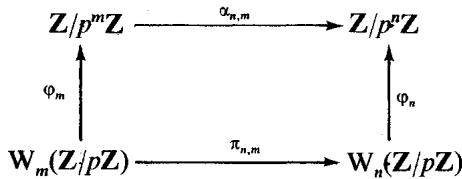
\includegraphics[keepaspectratio]{images/part001_40a15710.jpg}}

is commutative. It follows that \(\varphi = \varprojlim \varphi_n\) is an isomorphism of topological rings from \(\mathbf{W}(\mathbf{Z}/p\mathbf{Z}) = \varprojlim \mathbf{W}_n(\mathbf{Z}/p\mathbf{Z})\) onto \(\mathbf{Z}_p = \varprojlim \mathbf{Z}/p^n\mathbf{Z}\) (III, § 2, no. 12, example 3).

Let \(m\) and \(n\) be two integers \(\geqslant 1\) . By construction, one has an exact sequence of additive groups

\[
0 \longrightarrow \mathrm{W} (\mathrm{A}) \xrightarrow {\mathrm{V} ^ {m}} \mathrm{W} (\mathrm{A}) \xrightarrow {\pi_ {m}} \mathrm{W} _ {m} (\mathrm{A}) \longrightarrow 0.\tag{E}
\]

Passing to quotients, the endomorphism \(V^{n}\) of the additive group of W(A) defines a homomorphism \(V_{m}^{n}\) from the additive group of \(W_{m}(A)\) to that of \(W_{m+n}(A)\) . In other words, one has a commutative diagram

\pandocbounded{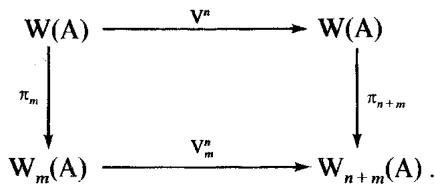
\includegraphics[keepaspectratio]{images/part001_7fe9268c.jpg}}

Passing to quotients, one deduces from the exact sequence (E) an exact sequence

\[
0 \longrightarrow \mathrm{W} _ {m} (\mathrm{A}) \xrightarrow {\mathrm{V} _ {m} ^ {n}} \mathrm{W} _ {n + m} (\mathrm{A}) \xrightarrow {\pi_ {n , n + m}} \mathrm{W} _ {n} (\mathrm{A}) \longrightarrow 0.\tag{E'}
\]

We have

\[
\mathrm{V} _ {m} ^ {n} [ a _ {0}, \dots , a _ {m - 1} ] = [ \underbrace {0 , \dots , 0} _ {n \text {   times }}, a _ {0}, \dots , a _ {m - 1} ],\tag{45}
\]

for every element \([a_0, \ldots, a_{m-1}]\) of \(\mathbf{W}_m(\mathbf{A})\) .

By prop. 3, c) of no. 5, one has FV \(^{m+1}\) (a) = p.V \(^{m}\) (a) for all a in W(A) and we consequently have F(V \(_{m+1}\) (A)) ⊂ V \(_{m}\) (A). By induction on n, it follows that F \(^{n}\) maps V \(_{n+m}\) (A) into V \(_{m}\) (A), and therefore defines, by passing to quotients, a ring homomorphism F \(^{n}\) :W \(_{n+m}\) (A) → W \(_{m}\) (A). By construction, we have a commutative diagram

\pandocbounded{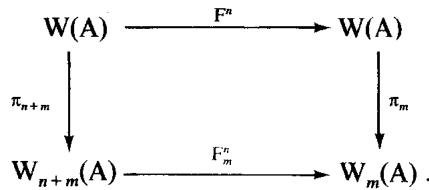
\includegraphics[keepaspectratio]{images/part001_14e9ec0a.jpg}}

Recall (no. 3) that the polynomial \(\mathbf{F}_i\) belongs to \(\mathbf{Z}[\mathbf{X}_0, \ldots, \mathbf{X}_{i+1}]\) for every integer \(i \geqslant 0\) ; the homomorphism \(\mathbf{F}_m^1\) from \(\mathbf{W}_{m+1}(\mathbf{A})\) to \(\mathbf{W}_m(\mathbf{A})\) is therefore made explicit as follows:

\[
\mathrm{F} _ {m} ^ {1} \left[ a _ {0}, \dots , a _ {m} \right] = \left[ \mathrm{F} _ {i} \left(a _ {0}, \dots , a _ {i + 1}\right) \right] _ {0 \leqslant i <   m}.\tag{46}
\]

Let \(\boldsymbol{a} \in \mathrm{W}_{m}(\mathbf{A})\) , \(\boldsymbol{a}' \in \mathrm{W}_{m}(\mathbf{A})\) and \(\boldsymbol{b} \in \mathrm{W}_{m+1}(\mathbf{A})\). The following formulas result by passing to quotients from Prop. 3 of No. 5:

\begin{enumerate}
\def\labelenumi{(\arabic{enumi})}
\setcounter{enumi}{46}
\tightlist
\item
\end{enumerate}

\[
\mathrm{F} _ {m} ^ {1} \left(\mathrm{V} _ {m} ^ {1} (\boldsymbol {a})\right) = p. \boldsymbol {a}\tag{48}
\]

\[
\mathrm{V} _ {m} ^ {1} (a \times \mathrm{F} _ {m} ^ {1} (b)) = \mathrm{V} _ {m} ^ {1} (a) \times b\tag{49}
\]

\[
\mathrm{V} _ {m} ^ {1} (a) \times \mathrm{V} _ {m} ^ {1} (a ^ {\prime}) = p. \mathrm{V} _ {m} ^ {1} (a \times a ^ {\prime})\tag{50}
\]

\[
\mathrm{V} _ {m} ^ {1} (\mathrm{F} _ {m} ^ {1} (b)) = \mu_ {m + 1} \times b
\]

\((\text{with } \boldsymbol{\mu}_{m+1} = [0, 1, 0, ..., 0]).\)

